\hypertarget{IU02}{\subsection{IU02 Página de ranking general}}


    \subsubsection{Pantalla de ranking}

    Después de obtener la información se mostrará el ranking general,
    ordenando a las empresas, de manera descendente, por el puntaje general obtenido.
    Este puntaje da prioridad tanto a la rentabilidad
    como a la liquidez de cada empresa sobre el endeudamiento y la rotación.

    \begin{figure}[H]
        \begin{center}
            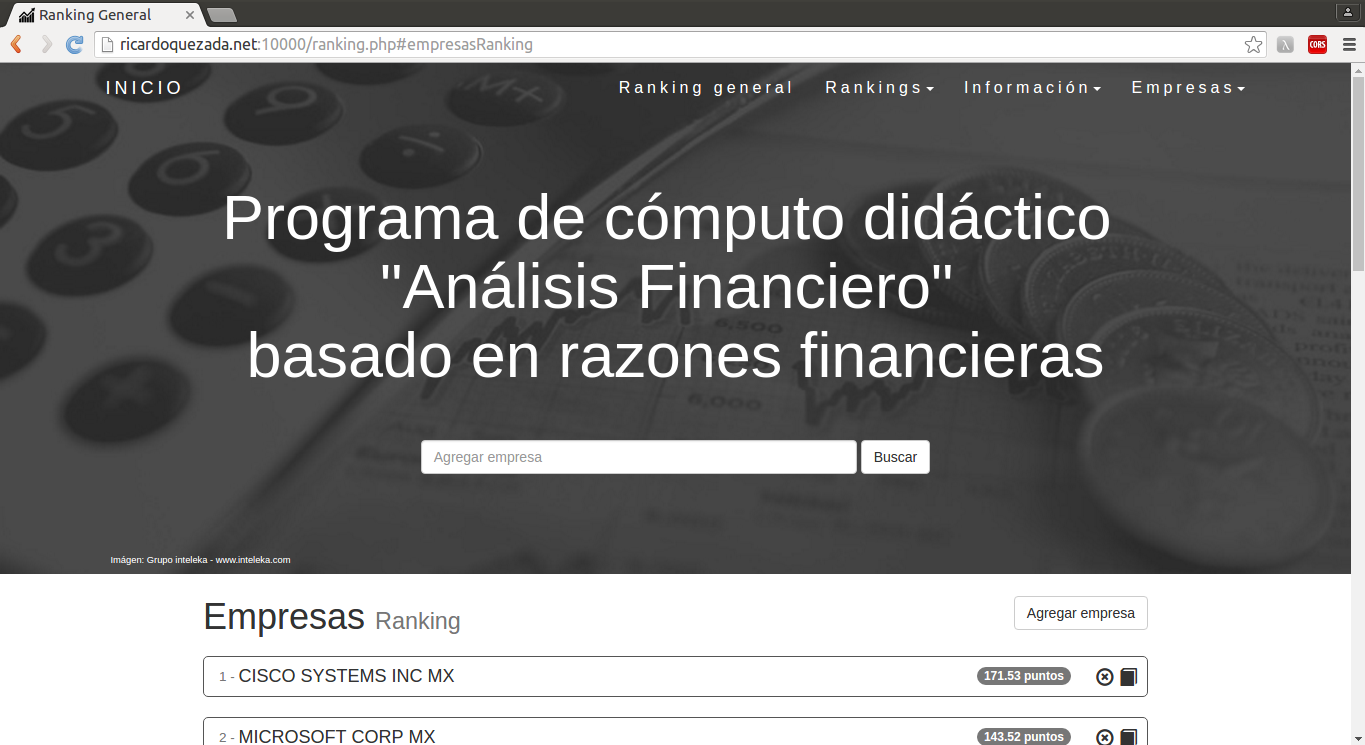
\includegraphics[scale=0.3]{pantallas/Ranking1}
            \caption{IU02/01 - Pantalla de ranking y búsqueda}
        \end{center}
    \end{figure}


    \subsubsection{Funcionalidades de ranking}

    Presione el botón con una cruz al centro para eliminar a esa empresa del análisis.
    Para obtener más información sobre una empresa, presione el ícono del libro correspondiente.

    Presione ``Agregar empresa'' para incluir en el análisis una empresa nueva, ajena al programa.
    Esta última opción abre en una nueva pestaña la página de agregar empresa.

    \begin{figure}[H]
        \begin{center}
            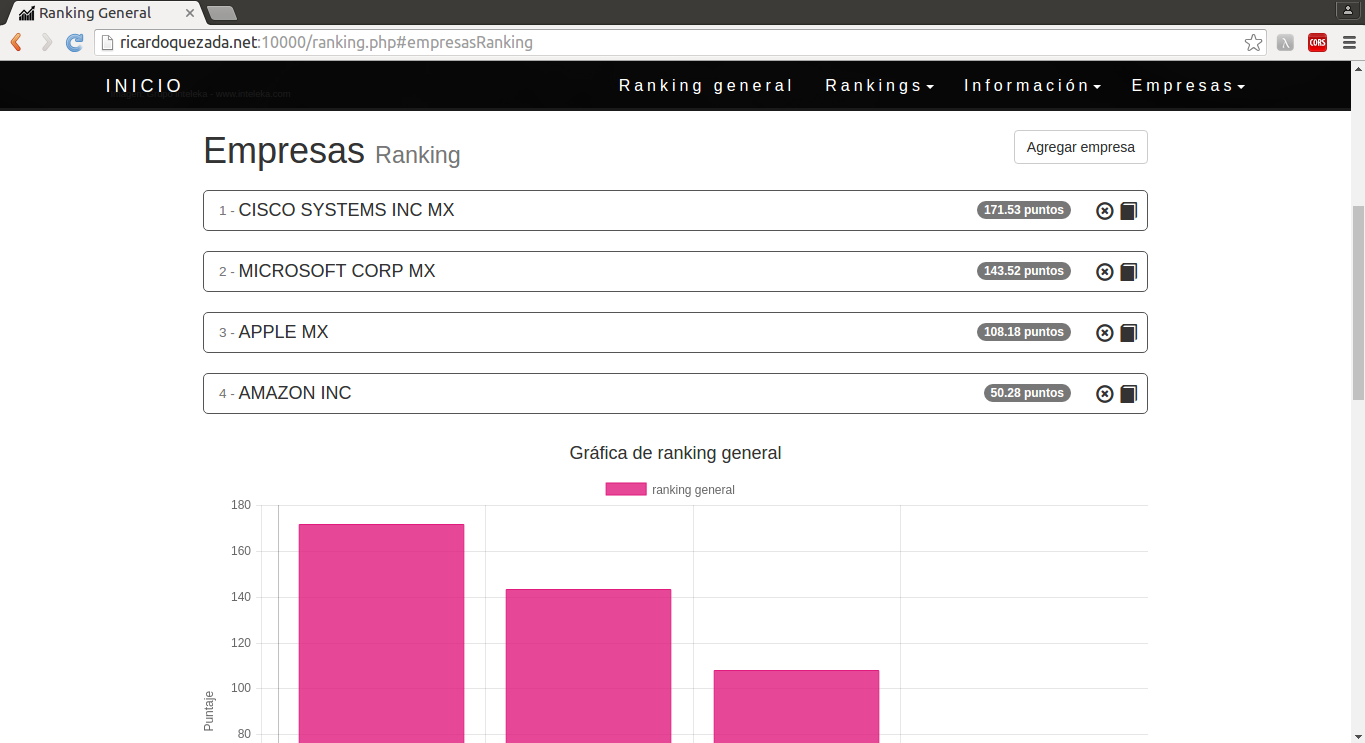
\includegraphics[scale=0.3]{pantallas/Ranking2}
            \caption{IU02/02 - Funcionalidades de ranking}
        \end{center}
    \end{figure}

    Introduzca el nombre de una nueva empresa en la barra de búsqueda para contemplarla en el análisis,
    las opciones irán mostrándose a medida que se escribe; para incluirla presione sobre su nombre 
    y despues sobre ``buscar''.

    \begin{figure}[H]
        \begin{center}
            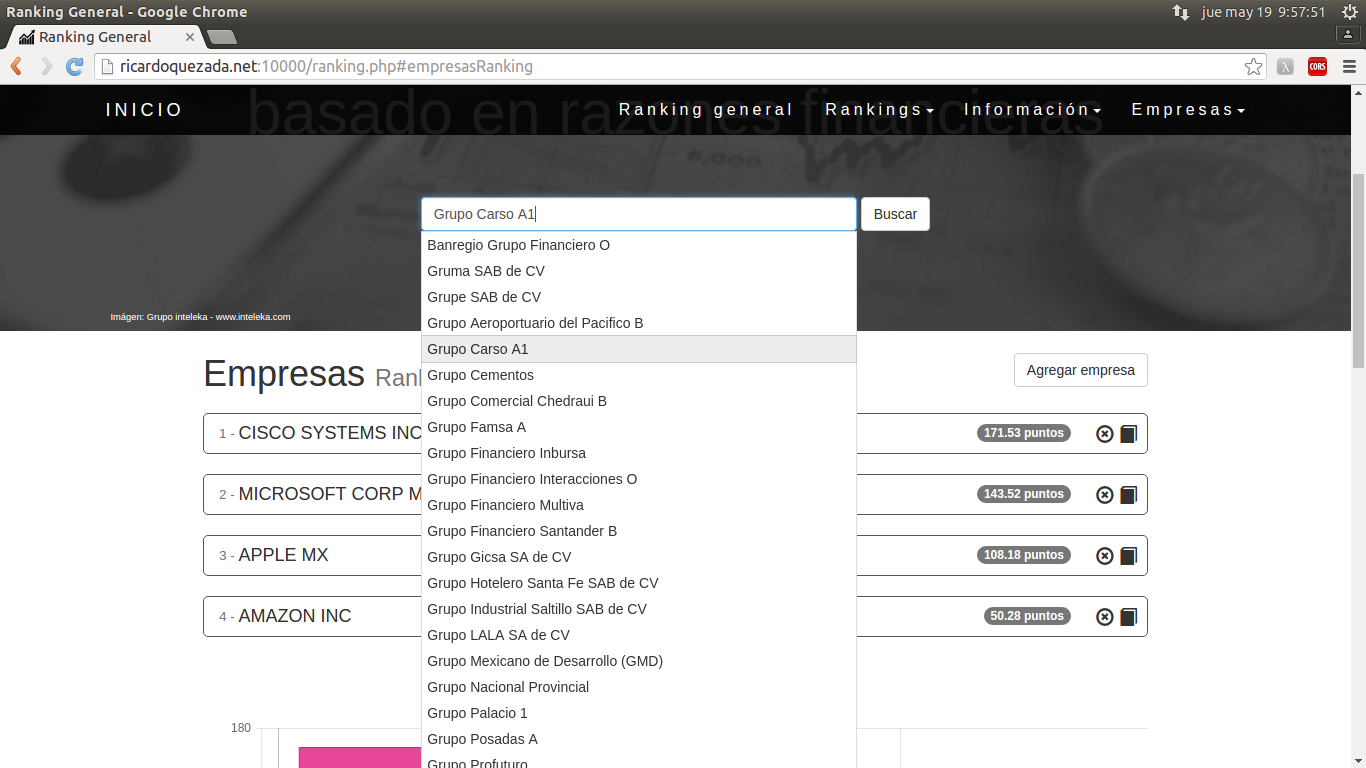
\includegraphics[scale=0.3]{pantallas/Ranking3}
            \caption{IU02/03 - Búsqueda de empresa}
        \end{center}
    \end{figure}


    \subsubsection{Funcionalidades de gráficas}

    Desplácese hacia abajo para ver una gráfica de barras el puntaje general obtenido por cada empresa.
    Pase el cursor sobre una barra para ver los puntos obtenidos y el nombre de la empresa correspondiente.

    \begin{figure}[H]
        \begin{center}
            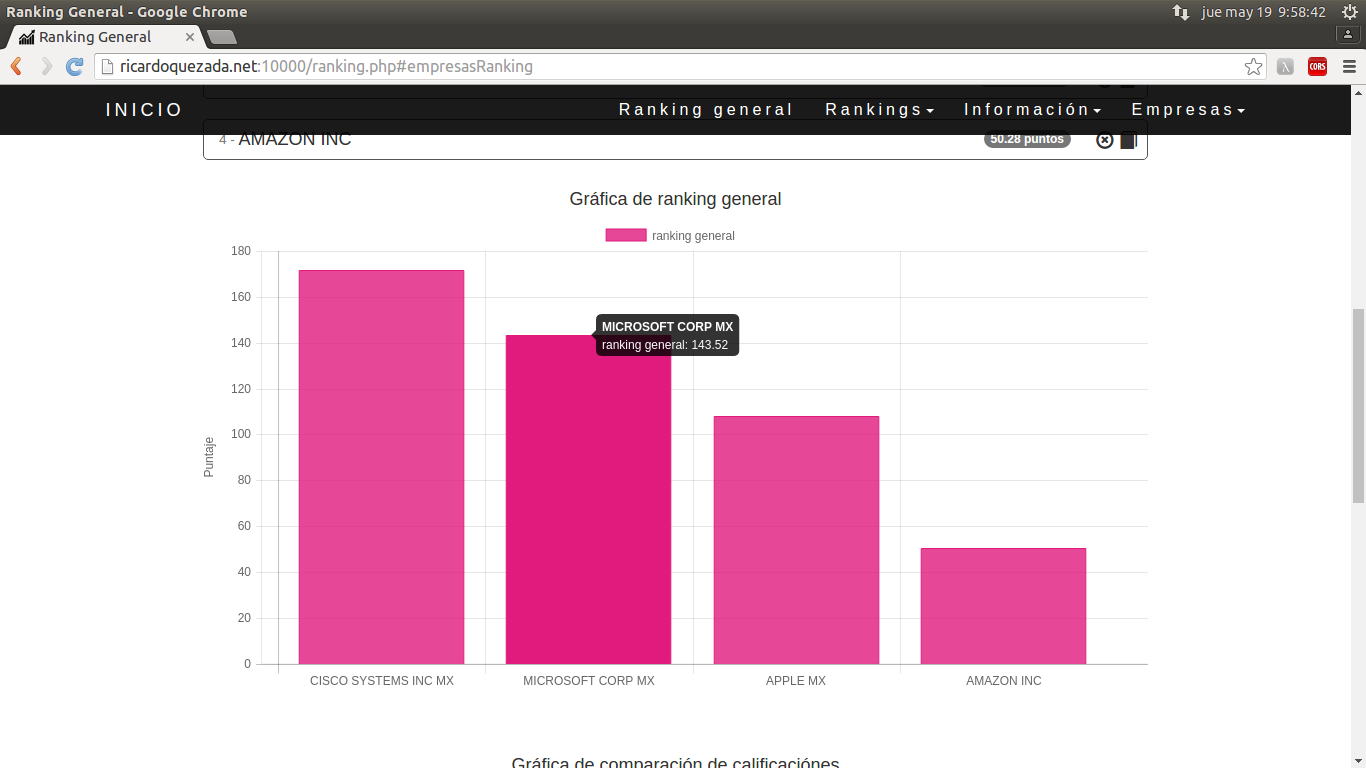
\includegraphics[scale=0.3]{pantallas/Ranking4}
            \caption{IU02/04 - Gráfica de barras de ranking general}
        \end{center}
    \end{figure}

    Desplácese más abajo para encontrar una gráfica de radar que compara el puntaje obtenido
    por cada empresa en los índices de rentabilidad, liquidez, rotaciones y endeudamiento.
    Entre mayor sea el área, mayor será su puntaje general.

    Presione sobre el nombre de una empresa para quitarla de la gráfica y observar a las otras
    con mayor detenimiento, la escala se reajustará automáticamente para las que queden
    seleccionadas y el nombre se verá tachado. Pulse sobre el nombre tachado
    para mostrarla nuevamente en la gráfica.

    Pase el cursor sobre un punto par observar el puntaje obtenido
    por esa empresa en el eje en que se encuatre.


    \begin{figure}[H]
        \begin{center}
            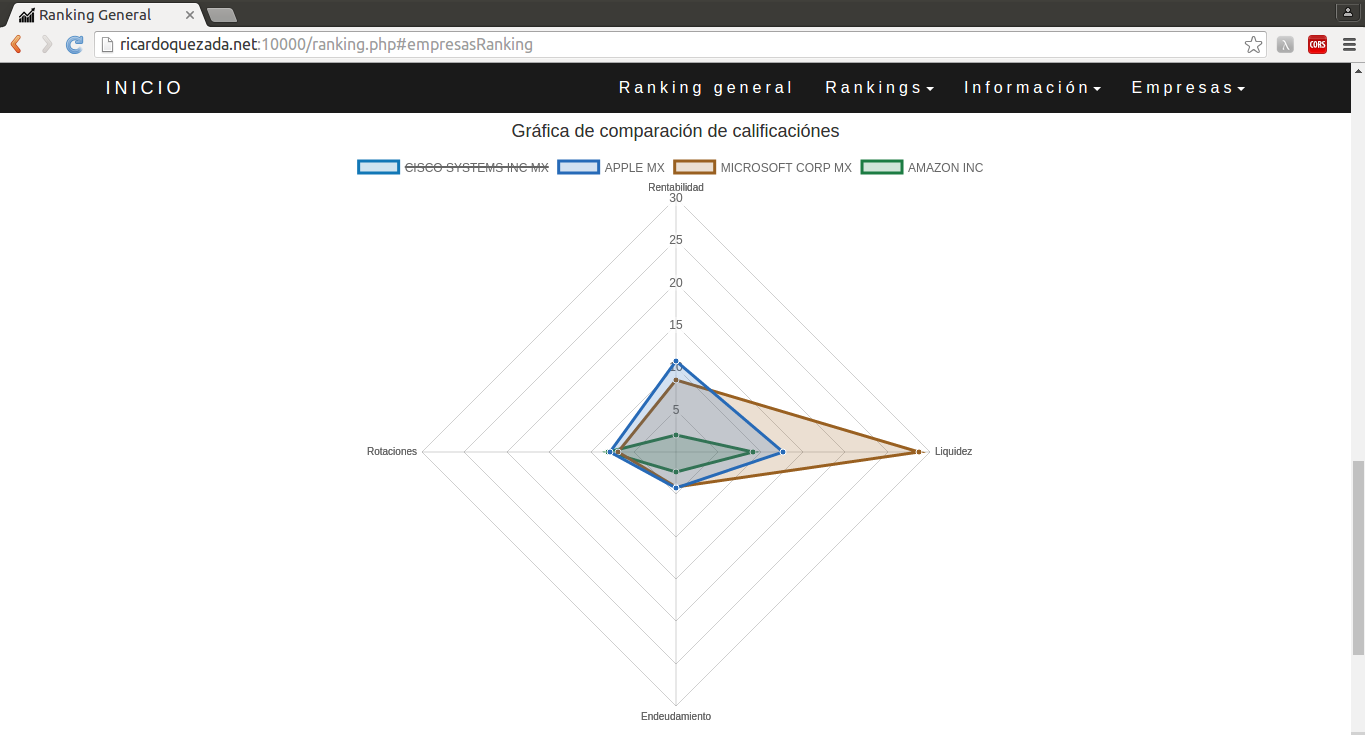
\includegraphics[scale=0.3]{pantallas/Ranking5}
            \caption{IU02/05 - Gráfica de radar de ranking general}
        \end{center}
    \end{figure}
